\documentclass[a4paper,10pt]{article}
\input{/home/frr/Dropbox/Modelos/Modelo_prova_latex/estilo_prova.tex}

\begin{document}


\professor{Fábio Rodrigues de la Rocha}
\turma{08655}
\codigodisciplina{ARA7560}
\disciplina{Sistemas Digitais Embarcados}
\data{14/03/2016}
\hlimite{20:20}
 \tarefa{3}
 
\lstset{language={}}          % Set your language (you can change the language for each code-block optionally)
\section{Introdução}

Nesta aula vamos estudar como funciona o sistema de Entradas e Saídas do lpc1768, especificamente a parte de entrada e saída digital.

O lpc1768 possui 5 portas de dados de 32 bits P0, P1, P2, P3 e P4. Mas para cada porta apenas alguns dos 32 bits podem ser utilizados. A razão para isso está na 
tentativa de manter uma compatibilidade com elementos anteriores da família ARM. (Detalhes vide página 118 do Manual do usuário)

\begin{lstlisting}
P0[30:0][1];  P0[14:12] are not available.
P1[31:0][2];  P1[2], P1[3], P1[7:5], P1[13:11] are not available.
P2[13:0]; 
P3[26:25];
P4[29:28]
\end{lstlisting}

Para cada porta existem registradores para indicar se vamos ler um valor, escrever um valor 1, escrever um valor 0 e fazer uma máscara para habilitar a alteração 
de um valor como mostra a tabela abaixo:

\begin{figure}[!htb]
 \centering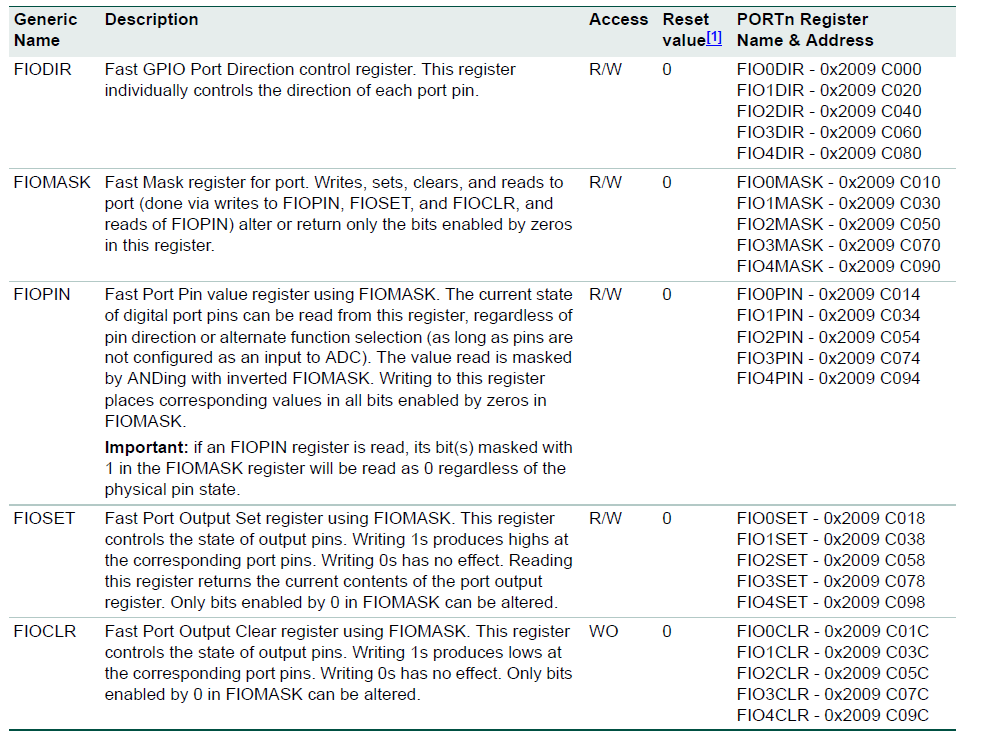
\includegraphics[width=\textwidth]{io}
\end{figure}


\begin{lstlisting}
#include "LPC17xx.h"
.
.

int main(void){
   SystemInit();
   LPC_GPIO1->FIODIR |= (1 << LED4_PIN);
   SysTick_Config(SystemCoreClock/(9600*4) - 1); /* Generate interrupt each 1 ms   */ 
 
   while(1){            
      LPC_GPIO1->FIOSET = (1 << LED4_PIN);
      Delay(10000);
      LPC_GPIO1->FIOCLR = (1 << LED4_PIN);
      Delay(10000);
   }
}
\end{lstlisting}

\subsection{Pinos que possuem mais de uma função}

Vários pinos possuem funções além de entrada/saída digital. Por exemplo podemos ter pinos TX, RX, SCL, SDA, etc. Para configurar se um pino será usado como 
entrada e saída ou será de função alternativa,  usamos o registrador PINSEL.

\begin{figure}[!htb]
 \centering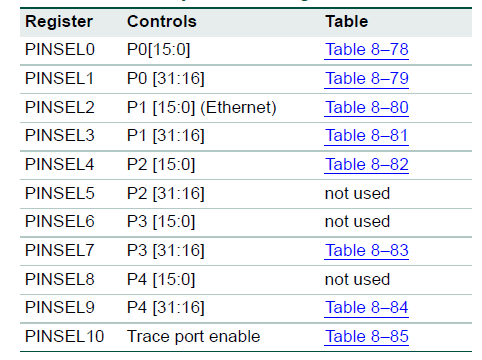
\includegraphics[width=0.4\textwidth]{pinsel_1}
\end{figure}
\begin{figure}[!htb]
 \centering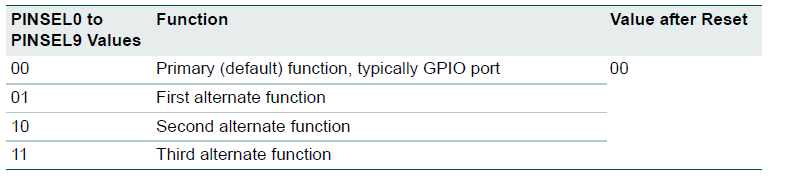
\includegraphics[width=0.5\textwidth]{pinsel_2}
\end{figure}


Veja o código abaixo:


\begin{lstlisting}

#include "LPC17xx.h"

#define LED_1 (1<<25)    //Porta 3.25
#define LED_2 (1<<26)    //      3.26

int main()
{    
    unsigned int cont,cont2;
    
    LPC_PINCON->PINSEL7=0;             //porta 3 como GPIO ->  
                                       
    LPC_GPIO3->FIODIR|=LED_2|LED_1;    //configura como saida
    
    LPC_GPIO3->FIOSET=LED_1;    //led apagado
    LPC_GPIO3->FIOCLR=LED_2;    //aceso
    
    while(1)
    {        
        if(LPC_GPIO3->FIOPIN&LED_1)
            {LPC_GPIO3->FIOCLR|=LED_1; LPC_GPIO3->FIOSET|=LED_2;}
        else
            {LPC_GPIO3->FIOSET|=LED_1; LPC_GPIO3->FIOCLR|=LED_2;}
        
        for(cont=0;cont<1524;cont++)
            for(cont2=0;cont2<65536;cont2++); //delay
    }
}
\end{lstlisting}


\end{document}

